%!TEX root = chi14grammatical.tex
\begin{figure*}[th]
	\begin{subfigure} {1.3\columnwidth}
			\centering
	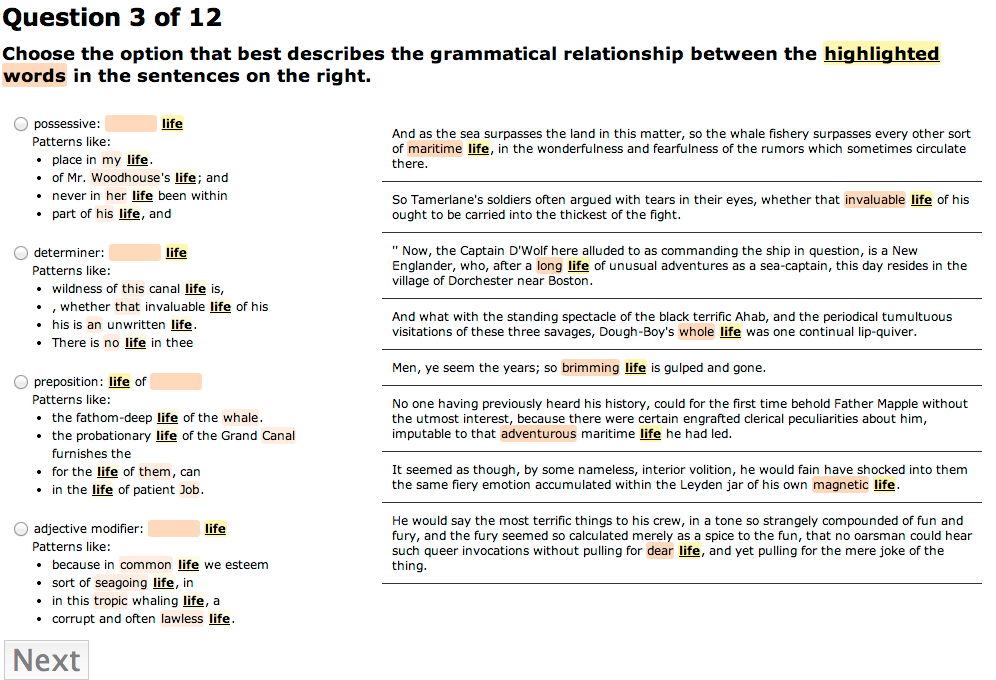
\includegraphics[width=1.2\columnwidth]{fig/task}
	\caption{\label{fig:task} An example of an identification task in the \emph{phrases} condition for the relationship \code{amod(life, \_\_\_)} (where different adjectives modify the noun `life'). The correct answer is `adjective modifier' (4th option), and the remaining 3 options are distractors.}
	\end{subfigure}
	\qquad\qquad\qquad
	\begin{subfigure}{0.7\columnwidth}
		\begin{subfigure}{0.7\columnwidth}
				\centering
		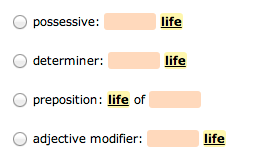
\includegraphics[width=0.9\columnwidth]{fig/baseline-choices}
	    \caption {The same options as they appear in the \emph{baseline} condition. \label{fig:baseline-choices}}
	    \end{subfigure}


	    \begin{subfigure}{0.7\columnwidth}
	    	\centering
	    	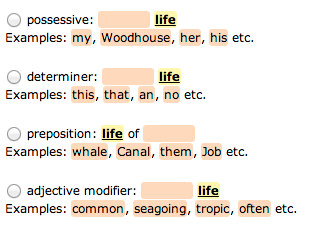
\includegraphics[width=0.9\columnwidth]{fig/words-choices}
	        \caption {The same options as they appear in the \emph{words} condition. \label{fig:words-choices}}
	    \end{subfigure}
	\end{subfigure}
\caption{\label{fig:choices} The appearance of the choices shown in the three experiment conditions.}
\end{figure*}

\section{Related Work}

Trees are the traditional representation of syntactic parses, so trees are often the focus of query input for collections of syntactically parsed data.   For instance, the Linguist's Search Engine \cite{resnik2005web} uses a query-by-example strategy in which a user types in an initial sentence in English, and the system produces a graphical view of a parse tree as output, in addition to a nested LISP expression of the same tree.  The user can either click on the tree or modify the LISP expression to generalize the query.    Similarly, the popular Stanford Parser includes Tregex, which as the name suggests,  allows for sophisticated regular expression search over syntactic tree structures, and Tsurgeon, which allows for manipulation of the trees extracted with Tregex \cite{levy2006tregex}.
%SPLICR also contains a graphical tree editor tool \cite{rehm2009sustainability}.
The Finite Structure Query tool for querying syntactically annotated corpora requires its queries to be stated in first order logic \cite{kepser2003finite}. In the Corpus Query Language \cite{jakubicek2010fast}, a query is a pattern of attribute-value pairs, where values can include regular expressions containing parse tree nodes and words.

Several approaches have adopted XML representations and the associated query language families of XPATH and SPARQL. For example, LPath augments XPath with additional tree operators to give it further expressiveness \cite{lai2010querying}.

A related approach is the query-by-example work seen in the past primarily in interfaces to database systems \cite{androutsopoulos1995natural}.
According to Shneiderman and Plaisant \cite{shneiderman2010designing}, query-by-example has largely fallen out of favor as a user interface design approach.  A downside of QBE is that the user must manipulate an example to arrive at the desired generalization.  At the same time, a related technique, auto-suggest, has become a widely-used approach in search user interfaces with strong support in terms of its usability \cite{hearst2009search}.   It is this approach that we investigate in this paper.

A final simple alternative approach is to name the relation of interest and show blanks where the words that satisfy the relation would appear as in \emph{X is the subject of Y} \cite{muralidharan2013supporting}; this is the baseline design tested below.
